\documentclass{exercise}

\setcounter{exercise}{5}
\newcommand{\topics}{Turing Machines, Undecidability}
\newcommand{\distdate}{23.11.2020}
\newcommand{\duedate}{06.12.2020}

\title{\line(1,0){415}\\
  Foundations of Computing II\\
  \Large Assignment \theexercise\ -- Solutions\\[1em]
  \large{\topics}\\
  \line(1,0){415}}

\lefttitle{Universit\"at Z\"urich\\Institut f\"ur Informatik\\[1em]
  \textsl{Student Name:}\\
  \textsl{Student Number:}}
\righttitle{Autumn 2020\\Sven Seuken\\Dennis Komm} 

\begin{document}

\maketitle

\begin{center}
  Distributed: \distdate\ -- Due Date: \duedate\\[1em]
  Upload your solutions to the OLAT system.\\[3em]
\end{center}

\task{Turing Machines}

Draw Turing machines (TMs) for the following languages and briefly explain how
your TMs work.

\subtask $L_1 = \{ a^kb^kw \mid k\in\nat^+\text{ and } w\in\{a,b\}^* \}$
  \begin{solution}
    Consider the following TM $M_1$ with $\text{Lang}(M_1)=L_1$.
    \begin{center}
      \begin{tikzpicture}[node distance=2.5cm and 2.2cm,x=2.5cm,y=2.2cm,font=\footnotesize]
      \node[state,initial] at (0,-1) (0) {$q_0$};
      \node[state] at (1,0) (1) {$q_1$};
      \node[state] at (2,0) (2) {$q_2$};
      \node[state] at (3,0) (3) {$q_3$};
      \node[state,accepting] at (0,-2) (4) {$q_4$};
      \path[->]
        (0) edge node[label]
        {\begin{mlabels}
         \tmlabel{a}{X}{\rmove}
         \end{mlabels}} (1)
        (1) edge node[label]
        {\begin{mlabels}
         \tmlabel{b}{Y}{\lmove}
         \end{mlabels}} (2)
        (1) edge[loop above] node[label]
        {\begin{mlabels}
         \tmlabel{a}{a}{\rmove}\\
         \tmlabel{Y}{Y}{\rmove}
         \end{mlabels}} (1)
        (2) edge node[label]
        {\begin{mlabels}
         \tmlabel{a}{a}{\lmove}
         \end{mlabels}} (3)
        (2) edge[bend left=10] node[yshift=3mm,label]
        {\begin{mlabels}
         \tmlabel{X}{X}{\rmove}
         \end{mlabels}} (0)
        (3) edge[bend left=20] node[label]
        {\begin{mlabels}
         \tmlabel{X}{X}{\rmove}
         \end{mlabels}} (0)
        (2) edge[loop above] node[label]
        {\begin{mlabels}
         \tmlabel{Y}{Y}{\lmove}
         \end{mlabels}} (2)
        (3) edge[loop above] node[label]
        {\begin{mlabels}
         \tmlabel{a}{a}{\lmove}
         \end{mlabels}} (3)
        (0) edge node[label]
        {\begin{mlabels}
         \tmlabel{Y}{Y}{\rmove}
         \end{mlabels}} (4);
      \end{tikzpicture}
    \end{center}
    The TM $M_1$ works as follows.  It starts by replacing the first $a$ by an
    $X$ which marks that this letter has already been processed.  If another
    letter than $a$ is found on the start position, the machine gets stuck in a
    non-accepting state (namely $q_0$).  After that, $M_1$ moves its head to the
    right over all subsequent $a$s and $Y$s.  If this is the first time, no $Y$
    is found.  The first $b$ that is found is marked by
    replacing it by a $Y$; this was the first not-yet-processed $b$.  While
    replacing $b$ by $Y$, the head is moved to the left, and the state
    $q_2$ is entered.  After that, the head is moved to the left over all $Y$s.
    If the rightmost $X$ is found, the head is moved to the right such that it
    is now positioned right of this $X$ and the state $q_0$ is entered.
    If an $a$ is found in $q_2$ instead, $M_1$ enters the state $q_3$, where it
    moves its head to the left over all remaining $a$s.  It again changes to 
    state $q_0$ if the rightmost $X$ is encountered.
  
    Finally, if $M_1$ finds a $Y$ right next to an $X$ in $q_0$, we know that it
    replaced the same number of $a$s and $b$s.  Therefore, it can enter the
    accepting state and halt; this way, $M_1$ neglects what is right of the last
    $Y$ it wrote.
  \end{solution}

\subtask $L_2 = \{ w0w \mid w \in\{1,2\}^* \}$

  \begin{solution}
    Consider the following TM $M_2$ with $\text{Land}(M_2)=L_2$.
    \begin{center}
      \begin{tikzpicture}[node distance=2.5cm and 2.2cm,x=2.5cm,y=2.2cm,font=\footnotesize]
      \node[state,initial] at (0,-1) (0) {$q_0$};
      \node[state] at (1,0) (1) {$q_1$};
      \node[state] at (2,0) (2) {$q_2$};
      \node[state] at (3,0) (3) {$q_3$};
      \node[state] at (4,0) (4) {$q_4$};
      \node[state] at (1,-2) (5) {$q_5$};
      \node[state] at (2,-2) (6) {$q_6$};
      \node[state] at (3,-2) (7) {$q_7$};
      \node[state] at (4,-2) (8) {$q_8$};
      \node[state] at (3,-1) (9) {$q_9$};
      \node[state,accepting] at (5,-1) (10) {$q_{10}$};
      \path[->]
        (0) edge node[label]
        {\begin{mlabels}
         \tmlabel{1}{X}{\rmove}
         \end{mlabels}} (1)
        (1) edge node[label]
        {\begin{mlabels}
         \tmlabel{0}{0}{\rmove}
         \end{mlabels}} (2)
        (1) edge[loop above] node[label]
        {\begin{mlabels}
         \tmlabel{1}{1}{\rmove} \\
         \tmlabel{2}{2}{\rmove}
         \end{mlabels}} (1)
        (2) edge node[label]
        {\begin{mlabels}
         \tmlabel{1}{X}{\lmove}
         \end{mlabels}} (3)
        (2) edge[loop above] node[label]
        {\begin{mlabels}
         \tmlabel{X}{X}{\rmove} \\
         \tmlabel{Y}{Y}{\rmove}
         \end{mlabels}} (2)
        (3) edge node[label]
        {\begin{mlabels}
         \tmlabel{0}{0}{\lmove}
         \end{mlabels}} (4)
        (3) edge[loop above] node[label]
        {\begin{mlabels}
         \tmlabel{X}{X}{\lmove} \\
         \tmlabel{Y}{Y}{\lmove}
         \end{mlabels}} (3)
        (4) edge node[label]
        {\begin{mlabels}
         \tmlabel{X}{X}{\rmove}
         \end{mlabels}} (0)
        (4) edge[loop above] node[label]
        {\begin{mlabels}
         \tmlabel{1}{1}{\lmove} \\
         \tmlabel{2}{2}{\lmove}
         \end{mlabels}} (4)
        (0) edge[swap] node[label]
        {\begin{mlabels}
         \tmlabel{2}{Y}{\rmove}
         \end{mlabels}} (5)
        (5) edge[swap] node[label]
        {\begin{mlabels}
         \tmlabel{0}{0}{\rmove}
         \end{mlabels}} (6)
        (5) edge[loop below] node[label]
        {\begin{mlabels}
         \tmlabel{1}{1}{\rmove} \\
         \tmlabel{2}{2}{\rmove}
         \end{mlabels}} (5)
        (6) edge[swap] node[label]
        {\begin{mlabels}
         \tmlabel{2}{Y}{\lmove}
         \end{mlabels}} (7)
        (6) edge[loop below] node[label]
        {\begin{mlabels}
         \tmlabel{X}{X}{\rmove} \\
         \tmlabel{Y}{Y}{\rmove}
         \end{mlabels}} (6)
        (7) edge[swap] node[label]
        {\begin{mlabels}
         \tmlabel{0}{0}{\lmove}
         \end{mlabels}} (8)
        (7) edge[loop below] node[label]
        {\begin{mlabels}
         \tmlabel{X}{X}{\lmove} \\
         \tmlabel{Y}{Y}{\lmove}
         \end{mlabels}} (7)
        (8) edge[swap] node[label]
        {\begin{mlabels}
         \tmlabel{Y}{Y}{\rmove}
         \end{mlabels}} (0)
        (8) edge[loop below] node[label]
        {\begin{mlabels}
         \tmlabel{1}{1}{\lmove} \\
         \tmlabel{2}{2}{\lmove}
         \end{mlabels}} (8)
        (0) edge node[label]
        {\begin{mlabels}
         \tmlabel{0}{0}{\rmove}
         \end{mlabels}} (9)
        (9) edge[loop right] node[label]
        {\begin{mlabels}
         \tmlabel{X}{X}{\rmove} \\
         \tmlabel{Y}{Y}{\rmove}
         \end{mlabels}} (9)
        (9) edge[swap,bend right=30] node[label]
        {\begin{mlabels}
         \tmlabel{B}{B}{\rmove}
         \end{mlabels}} (10);
      \end{tikzpicture}
    \end{center}
    The overall idea behind $M_2$ is to compare the strings it finds before and
    after the $0$ symbol by symbol.  As before, the machine is constructed in
    such a way that it gets stuck in a non-accepting state if it finds more
    than one $0$.  The same happens if it does not find any $0$ at all.
  
    Starting from $q_0$, $M_2$ moves either to $q_1$ or $q_5$, depending on whether
    it reads a $1$ or a $2$.  Depending on this state, it knows whether it must
    find another $1$ or $2$ in the second part of the word.  After the first $0$
    it finds, it moves over all letters that are already marked; the marking is
    done by replacing $1$s by $X$s and $2$s by $Y$s.  Then, it marks
    another $1$ or $2$, and moves back to the field that is next to the one it
    marked in the first part of the word.  It is then back in $q_0$ and the
    process is repeated.
  
    Finally, if $M_2$ finds a $0$ in $q_0$, it moves to $q_9$.  This can also
    happen if no $1$ or $2$ are found at all, which ensures that the word $0$ is
    accepted.  Then it moves over all symbols that are already marked, that is,
    $X$s and $Ys$.  $M_2$ only accepts if it finds a blank $B$ after that.  If it
    encounters a letter different from $B$ after reading all $X$s and $Y$s, the
    word is not accepted as the part behind the $0$ is longer than the one
    before.  If the first part is longer, $M_2$ gets stuck before, namely when it
    encounters a $B$ either in $q_2$ or $q_6$.
  \end{solution}

\nosubtask \textit{Hint:} It is sufficient to construct TMs with one tape each.
Recall that you can assume that the input word only contains letters from the
implicitly given alphabet; for instance, in a), there are only letters $a$ and
$b$ on the tape at the beginning.

\task{Turing Machines and Configurations}

Consider the following TM $M$ with $\text{Lang}(M)\subseteq\{0,1\}^*$.
\begin{center}
  \begin{tikzpicture}[x=3cm,y=2.2cm]
    \node[state]           at (0,0)  (2) {$q_2$};
    \node[state]           at (-1,0) (1) {$q_1$};
    \node[state,initial]   at (-2,0) (0) {$q_0$};
    \node[state]           at (1,0)  (3) {$q_3$};
    \node[state,accepting] at (2,0)  (4) {$q_4$};
    \path[->]
      (0) edge[loop above] node[label]
      {\begin{mlabels}
       \tmlabel{0}{0}{\rmove}
       \end{mlabels}} (0)
      (0) edge node[label]
      {\begin{mlabels}
       \tmlabel{1}{Y}{\lmove}
       \end{mlabels}} (1)
      (2) edge[loop above] node[label]
      {\begin{mlabels}
       \tmlabel{X}{X}{\rmove}\\
       \tmlabel{Y}{Y}{\rmove}
       \end{mlabels}} (2)
      (2) edge[bend left] node[label]
      {\begin{mlabels}
       \tmlabel{1}{Y}{\lmove}
       \end{mlabels}} (1)
      (1) edge[bend left] node[label]
      {\begin{mlabels}
       \tmlabel{0}{X}{\rmove}
       \end{mlabels}} (2)
      (1) edge[loop above] node[label]
      {\begin{mlabels}
       \tmlabel{X}{X}{\lmove}\\
       \tmlabel{Y}{Y}{\lmove}
       \end{mlabels}} (1)
      (2) edge node[label]
      {\begin{mlabels}
       \tmlabel{\blank}{Z}{\lmove}
       \end{mlabels}} (3)
      (3) edge[loop above] node[label]
      {\begin{mlabels}
       \tmlabel{X}{X}{\lmove}\\
       \tmlabel{Y}{Y}{\lmove}\\
       \tmlabel{Z}{Z}{\lmove}
       \end{mlabels}} (3)
      (3) edge node[label]
      {\begin{mlabels}
       \tmlabel{\blank}{Z}{\rmove}
       \end{mlabels}} (4);
    \end{tikzpicture}
\end{center}

\subtask Give the computation of $M$ (\ie, the unique sequence of configurations) on
  the following words; indicate when $M$ gets stuck or accepts.

  \begin{taskitems}
    \item $01$
    \item $001$
    \item $101$
    \item $00111$
  \end{taskitems}

  \begin{solution}
    \begin{taskitems}
		  \item $q_001 \tmmove 0q_01 \tmmove q_10Y \tmmove Xq_2Y \tmmove XYq_2\blank \tmmove Xq_3YZ$\\[1mm]
			      \hspace*{0.66cm} $\tmmove q_3XYZ \tmmove q_3\blank XYZ \tmmove Zq_4XYZ$ \hfill and $M$ accepts
		  \item $q_0001 \tmmove 0q_001 \tmmove 00q_01 \tmmove 0q_10Y \tmmove 0Xq_2Y \tmmove 0XYq_2\blank$\\[1mm]
						\hspace*{0.85cm} $\tmmove 0Xq_3YZ \tmmove 0q_3XYZ\tmmove q_30XYZ$ \hfill and $M$ gets stuck
			\item $q_0101 \tmmove q_1\blank Y01$ \hfill and $M$ gets stuck
      \item $q_000111 \tmmove 0q_00111 \tmmove 00q_0111 \tmmove 0q_10Y11 \tmmove 0Xq_2Y11 \tmmove 0XYq_211$\\[1mm]
			      \hspace*{1.25cm} $\tmmove 0Xq_1YY1 \tmmove 0q_1XYY1 \tmmove q_10XYY1 \tmmove Xq_2XYY1$\\[1mm]
			      \hspace*{1.25cm} $\tmmove XXq_2YY1 \tmmove XXYq_2Y1 \tmmove XXYYq_21 \tmmove XXYq_1YY$\\[1mm]
			      \hspace*{1.25cm} $\tmmove XXq_1YYY \tmmove Xq_1XYYY \tmmove q_1XXYYY$\\[1mm]
						\hspace*{1.25cm} $\tmmove q_1\blank XXYYY$  \hfill and $M$ gets stuck
    \end{taskitems}
  \end{solution}

\subtask Describe $\text{Lang}(M)$ in words.

  \begin{solution}
    $\text{Lang}(M)$ does not contain the empty word $\varepsilon$, because it cannot
		transition from its start state $q_0$ to its accepting state $q_4$ if the tape is empty (\ie, only
		contains blanks).
    
		Otherwise, it runs over all $0$s without changing them.  If a $1$ is encountered, it
		is marked by replacing it by $Y$; $M$ changes to $q_1$ in this case.  After that,
		$M$ runs back over all $X$s and $Y$s until it finds the rightmost $0$ (if there is
		one).  This $0$ is then marked by replacing it by $X$; $M$ changes to $q_2$.
		After this first iteration, the rightmost $0$ and the leftmost $1$ are marked.
		$M$ continues this way.  Just as seen in ii.\ and iv., $M$ gets stuck if the
		numbers of $0$s and $1$s encountered do not match.  It does not accept
		any word where a $0$ follows a $1$.

		We conclude that $\text{Lang}(M)=\{0^n1^n\mid n\in\nat^+\}$.
  \end{solution}

\task{Diagonalization}

Consider the following two languages.
\begin{align*}
  L_{\text{diag},1} &= \{ w\in\{0,1\}^* \mid w = w_{2i} \text{ and } M_i \text{ does not accept } w_{2i} \}\;,\\
  L_{\text{diag},2} &= \{ w\in\{0,1\}^* \mid w = w_i \text{ and } M_{2i} \text{ does not accept } w_i \}\;.
\end{align*}
Here, we again assume that $M_i$ is the $i$th TM in a fixed ordering
and $w_i$ is the $i$th binary word in a fixed ordering over some given alphabet.
We see that both of these languages are constructed in a way that reminds us
of the language $L_{\text{diag}}$; the only part that is different is that we
do not speak about the main diagonal of the corresponding table, but two different
diagonals that are shallower or steeper, respectively.

\subtask For one of the two languages, prove that it is not recursively enumerable.

  \begin{solution}
    The language $L_{\text{diag},1}$ is not recursively enumerable.  We can prove
    this claim analogously to the proof that shows that $L_{\text{diag}}$ (that is,
    the original diagonal language) is not recursively enumerable.
    
    Towards contradiction, assume $L_{\text{diag},1}$ were recursively
    enumerable.  This means that there is some TM $M$ that accepts this
    language, that is, $\text{Lang}(M)=L_{\text{diag},1}$.  $M$ must be in the list of
    all TMs, thus $M=M_i$ for some $i\in\nat^+$.
    \begin{itemize}
      \item Assume $w_{2i}\in L_{\text{diag},1}$.  Then, $M_i$ accepts $w_{2i}$, because
        $M_i$ accepts $L_{\text{diag},1}$.  However, by the definition of
        $L_{\text{diag},1}$, $w_{2i}$ cannot be accepted by $M_i$, because
        $L_{\text{diag},1}$ only contains the words $w_j$ that are not accepted
        by $M_j$, for any $j\in\nat^+$; thus, $w_{2i}\notin\text{Lang}(M_i)=L_{\text{diag},1}$.
      \item Assume $w_{2i}\notin L_{\text{diag},1}$.  Then, $M_i$ does not
        accept $w_{2i}$; but by definition, in this case $w_{2i}$ must be in
        $L_{\text{diag},1}$.
    \end{itemize}
    In both cases, we get a contradiction; because we just showed
    \[ w_{2i}\in L_{\text{diag},1} \iff w_{2i}\notin L_{\text{diag},1}\;. \]
    Therefore, the TM $M$ cannot exist,
    which directly implies that $L_{\text{diag},1}$ is not recursively enumerable.
  \end{solution}

\subtask For the other language, explain why the same argument as in a) is not
  valid to prove that this language is also not recursively enumerable.

  \begin{solution}
    For the language $L_{\text{diag},2}$, we cannot give a similar argument,
    because we do not consider every TM in the list of all TMs, but only every
    second.  This does not allow for a contradiction in the above way, because
    the TM for $L_{\text{diag},2}$ could be the $j$th TM and there is no $i$ such
    that $j=2i$.  Therefore, the hypothesis that $w_j$ is in $\text{Lang}(M_j)$
    does not lead to a contradiction since it is not necessary that $w_j$
    is not in $L_{\text{diag},2}$.

    However, note that this does not imply that $L_{\text{diag},2}$ is
    recursively enumerable.  It only means that this particular proof does not
    work.
  \end{solution}

\task{More Diagonalization}

Let $L$ be some infinite language over $\{0,1\}$.  Explain how we can
identify a subset $L_{\text{diag},L}$ of $L$ such that $L_{\text{diag},L}$
is not recursively enumerable.

\begin{solution}
  Once more, let $M_i$ be the $i$th TM in some fixed ordering.  The idea
  of the following construction is to design $L_{\text{diag},L}$ relative
  to $L$ as
  \begin{align*}
    L_{\text{diag},L} =  \{w\in\{0,1\}^*\mid &\, w=w_i\text{ is the $i$th word in $L$ for some $i\in\nat^+$}\\
                                             &\, \text{and $M_i$ does not accept $w_i$}\}\;.
  \end{align*}

  We can now again argue similarly as in the original proof.  For a contradiction,
  suppose that $L_{\text{diag},L}$ were recursively enumerable, and let $M$ be a TM
  with $L_{\text{diag},L}=\text{Lang}(M)$; there has to be an $i\in\nat^+$ with
  $M=M_i$, and therefore $L_{\text{diag},L}=\text{Lang}(M_i)$.  This time, consider
  the $i$th word $w_i$ in $L$.
  \begin{itemize}
    \item Assume $w_i\in L_{\text{diag},L}$.  Then, $M_i$ accepts $w_i$, because
      $M_i$ accepts $L_{\text{diag},L}$.  However, $w_i$ cannot be accepted by $M_i$, because
      $L_{\text{diag},L}$ only contains the words $w_j$ from $L$ that are not accepted
      by $M_j$, for every $j\in\nat^+$; thus, $w_i\notin\text{Lang}(M_i)=L_{\text{diag},L}$.
    \item Assume $w_i\notin L_{\text{diag},L}$.  Then, $M_i$ does not
      accept $w_i$; but in this case $w_i$ must be in $L_{\text{diag},L}$.
  \end{itemize}
  We therefore obtain
  \[ w_i\in L_{\text{diag},L} \iff w_i\notin L_{\text{diag},L}\;, \]
  which is a contradiction.  As a consequence, $L_{\text{diag},L}$ cannot
  be recursively enumerable.
\end{solution}

\task{Reductions}

$L_{\text{diag}}$ was the first language for which we showed that it is not recursively
enumerable and thus not recursive.  To prove that there are other
languages that are not recursively enumerable or not recursive, we use reductions.

In the lecture, we showed that $L_{\text{U}}$ is not recursive and argued as
follows.  We know that, if $L_{\text{U}}$ were recursive, then also its
complement $\overline{L}_{\text{U}}$ would be recursive.  Thus, if we succeed
in showing that $\overline{L}_{\text{U}}$ is not recursive, then $L_{\text{U}}$
cannot be recursive.  We then reduced $L_{\text{diag}}$ to
$\overline{L}_{\text{U}}$, that is, the problem of deciding whether a given
word is in $L_{\text{diag}}$ to deciding whether some word is in
$\overline{L}_{\text{U}}$.  If then we would have a TM $\overline{U}^*$ for deciding
$\overline{L}_{\text{U}}$ (that is, if this language were recursive), we could
use it to decide $L_{\text{diag}}$ (that is, this language would also be
recursive).

\nosubtask We want to slightly modify the original proof, but essentially prove the same statement.

\subtask Formally define the language $\overline{L}_{\text{diag}}$, that is, the complement of $L_{\text{diag}}$.

  \begin{solution}
    $\overline{L}_{\text{diag}}$ contains all binary strings $w$ for which it holds that, if $w$ is the
    $i$th binary string, the TM $M_i$ accepts $w$.  Formally, we have
    \[ \overline{L}_{\text{diag}} = \{ w\in\{0,1\}^* \mid w = w_{i} \text{ and } M_i \text{ accepts } w_{i} \}\;. \]
  \end{solution}

\subtask Prove that $\overline{L}_{\text{diag}}$ is recursively enumerable.

  \begin{solution}
		We describe a TM $\overline{D}$ that accepts all strings in
		$\overline{L}_{\text{diag}}$.  $\overline{D}$ is not guaranteed to halt if
		a given string is not in $\overline{L}_{\text{diag}}$ (in this case, this
		word is in $L_{\text{diag}}$).  However, $\overline{D}$ accepts all words
		(and thus halts) that are in $\overline{L}_{\text{diag}}$.

		For a given input $w$, $\overline{D}$ computes the index $i$ of this word;
		thus, $w=w_i$ for some $i\in\nat^+$.  Then, $\overline{D}$ computes the
		index $i$ of the $i$th TM $M_i$.  After that, $\overline{D}$ simulates $M_i$
    on $w_i$.

    If $M_i$ enters an accepting state, $\overline{D}$ also accepts; if $M_i$ gets
    stuck, $\overline{D}$ also gets stuck by entering a state that does not have any outgoing
    transition.  If $M_i$ runs forever, $\overline{D}$ also runs forever since the simulation
    of $M_i$ on $w_i$ never ends.

    \begin{itemize}
      \item If $w_i$ is accepted by $M_i$, $\overline{D}$ will eventually accept by definition.
        In this case, $w=w_i$ is in $\overline{L}_{\text{diag}}$.
      \item Otherwise $\overline{D}$ will either reject $w=w_i$ by getting stuck or never halt.
        In this case, $w=w_i$ is not in $\overline{L}_{\text{diag}}$.
    \end{itemize}
  \end{solution}

\subtask Reduce $\overline{L}_{\text{diag}}$ to $L_{\text{U}}$ to give an alternative proof
  that $L_{\text{U}}$ is not recursive.

  \begin{solution}
		Assume that $U^*$ is a TM for $L_{\text{U}}$ that always halts.  We
		design a TM $\overline{D}^*$ for $\overline{L}_{\text{diag}}$
		analogously to the original proof.  The idea is given in the following
		figure.
    \begin{center}
      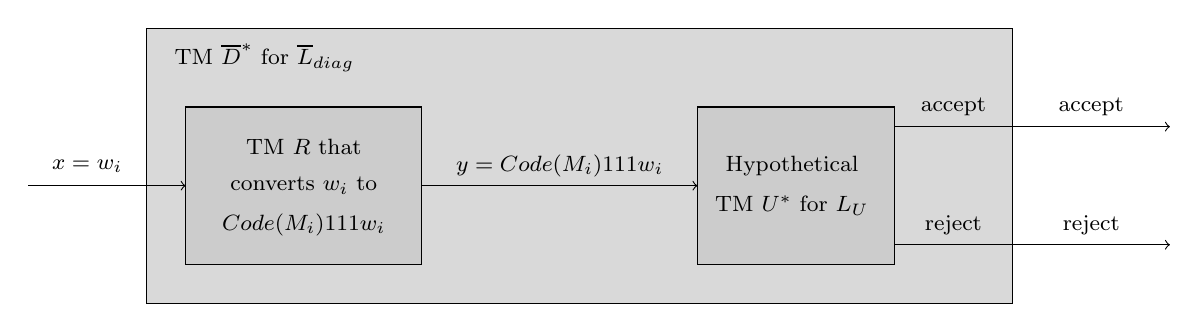
\begin{tikzpicture}[font=\footnotesize]
        \draw[fill=gray!30] (-1.5,0)  rectangle (9.5,3.5);
        \draw[fill=gray!40] (5.5,2.5) rectangle (8,0.5);
        \draw[fill=gray!40] (-1,2.5)  rectangle (2,0.5);
        \node at (0,3.125)     {TM $\overline{D}^*$ for $\overline{L}_{\text{diag}}$};
        \node at (6.7,1.75)    {Hypothetical};
        \node at (6.7,1.25)    {TM $U^*$ for $L_{\text{U}}$};
        \node at (0.5,2)       {TM $R$ that};
        \node at (0.5,1.5)     {converts $w_i$ to};
        \node at (0.5,1)       {$\text{Code}(M_i)111w_i$};
        \node at (-2.25,1.75)  {$x=w_i$};
        \node at (3.75,1.75)   {$y=\text{Code}(M_i)111w_i$};
        \draw[->] (-3,1.5) -- (-1,1.5);
        \draw[->] (2,1.5)  -- (5.5,1.5);
        \draw[->] (8,0.75) -- (11.5,0.75);
        \draw[->] (8,2.25) -- (11.5,2.25);
        \node at (8.75,2.5) {accept};
        \node at (8.75,1)   {reject};
        \node at (10.5,2.5) {accept};
        \node at (10.5,1)   {reject};
      \end{tikzpicture}
    \end{center}
    The description of $\overline{D}^*$ and all arguments can also be given in a way
		similar to the original construction.
    We first give $x=w_i$ to a TM $R$ that computes the index $i$ and the $i$th TM $M_i$.
    $R$ then outputs the word $y=\text{Code}(M_i)111w_i$, which is a valid
    input for $U^*$.  It expects the part before the three $1$s to
    be the encoding of a TM and the string behind them to be some binary word.  Then,
    by the definition of $L_{\text{U}}$, $U^*$ will accept if and only if
    the TM $M_i$ that is encoded accepts $w_i$, which is the case if and only if
    $x=w_i$ is in $\overline{L}_{\text{diag}}$.  It other words, we have
    \[ x\in \overline{L}_{\text{diag}} \iff y\in L_{\text{U}} \;, \]
    and we can simply give the same answer to decide whether $x$ is in
    $\overline{L}_{\text{diag}}$.  Consequently, $\overline{D}^*$ decides
    $\overline{L}_{\text{diag}}$, which is a contradiction to the fact that
    $\overline{L}_{\text{diag}}$ is not recursive (which in turn immediately follows
    from the fact that $L_{\text{diag}}$ is not recursive).
  \end{solution}

\task{More Reductions}

Consider the two languages
\begin{align*}
  L_3 &=\{(M,M',w) \mid M \text{ and } M' \text{ are TMs and } w\in \text{Lang}(M)\cap \text{Lang}(M')\}\;,\\
  L_4 &=\{(M,M',w) \mid M \text{ and } M' \text{ are TMs and } w\in \text{Lang}(M)\cup \text{Lang}(M')\}\;.
\end{align*}

\subtask Show that neither $L_3$ nor $L_4$ is recursive by giving a reduction from $L_{\text{U}}$.

  \begin{solution}
    Suppose $L_3$ were recursive.  Then we can use a hypothetical TM $M_3^*$
    for $L_3$ to  decide $L_{\text{U}}$.  Any input $x=(M,w)$, for which we
    want to decide whether it is in $L_{\text{U}}$, is mapped to an input
    $(M,M,w)$ that is given to $M_3^*$.  If and only if $(M,M,w)\in L_3$,
    and consequently $M_3^*$ accepts this  input, both given TMs that are
    encoded in it (\ie, the TM $M$) accept
    $w$; thus, $w\in \text{Lang}(M)=\text{Lang}(M)\cap \text{Lang}(M)$.  As a
    result, we have
    \[ (M,w)\in L_{\text{U}} \iff (M,M,w)\in L_3\;, \]
    and therefore can take the answer of $M^*_3$ to decide whether $x\in L_{\text{U}}$.

    We can use the same construction to give a reduction to $L_4$ instead of $L_3$.
  \end{solution}

\subtask Give a reduction from $L_3$ to $L_{\text{U}}$.  Do so by using that the two TMs $M$ and $M'$
    can be simulated sequentially on the same word.

  \begin{solution} %% input pruefen!
		Suppose $L_{\text{U}}$ were recursive and let TM $U^*$ denote the
		corresponding TM.  Consider an input $x=(M,M',w)$ for $L_3$.  We design a TM
		$M''$ that first simulates $M$ on any given input $y$.  If $M$ accepts $y$,
		$M''$ simulates $M'$ on $y$.  If $M'$ also accepts $y$, $M''$ accepts.  If
		$M$ or $M'$ rejects $y$, $M''$ rejects.  If $M$ or $M'$ runs forever on
		$y$, $M''$ also runs forever, because its simulation never ends.  Then
		$(M'',w)$ is given to $U^*$.  If and only if $(M'',w)\in L_{\text{U}}$, and
		hence $U^*$ answers that $M''$ accepts $w$, we know that both $M$ and $M'$
		accept $w$.  Therefore, $w\in \text{Lang}(M)\cap\text{Lang}(M')$, \ie
		$(M,M',w)\in L_3$ and we have
		\[ (M,M',w)\in L_3 \iff (M'',w)\in L_{\text{U}}\;, \]
    and we can take the answer of $U^*$ to decide whether $x\in L_3$.
  \end{solution}

\subtask Point out where we run into problems for a similar reduction as in exercise part
  b) from $L_4$ to $L_{\text{U}}$.  How can we deal with this problem?

  \begin{solution}
    We cannot follow a similar approach for $L_4$.  First simulating $M$ and then $M'$ may lead
    to $M$ not halting although $M'$ would accept.  This is fine for exercise part b) where the
    condition is that both TMs accept $w$, but here it is sufficient if one does.
    As one possible solution to this problem, $M''$ does not
    simulate $M$ and $M'$ sequentially but in parallel on the same input.  This is achieved
    by a diagonalization argument, somewhat similar to that which allows us to enumerate
		the rational numbers.  First, $M$ is simulated doing its first computational step on
    $w$; then $M'$ is simulated doing its first two steps on $w$; then again $M$ is simulated with
    its first three steps on $w$ etc.  If $M$ or $M'$ accepts $w$ after a finite number
    of computational steps, $w$ will eventually be accepted.  $(M'',w)$ is then again given
    to the hypothetical TM $U^*$ for $L_{\text{U}}$.
  \end{solution}

\task{Yet Another Reduction}

Consider TMs with exactly one accepting state and some fixed way to encode them.  Using a reduction,
show that the language
\begin{align*}
  L_5 = \{(M,w,i) \mid {}& M \text{ is a TM that visits its } i\text{th}\\
                         & \text{state at least once when processing } w \}\;.
\end{align*}
is not recursive.

\begin{solution}
  Suppose, $L_5$ were recursive.
  We give a reduction from $L_{\text{U}}$ to $L_5$.  Consider an input
  $x=(M,w)$ for $L_{\text{U}}$.  Since $M$ has one accepting state, we can compute its
  index, say $j\in\nat$.   Then we create an input $(M,w,j)$ that is given to the hypothetical
  TM $M^*_5$ which decides $L_5$.  If $M^*_5$ accepts $(M,w,j)$, this means that
  the $j$th state of $M$ is visited when $M$ gets $w$ as input.  Since the $j$th
  state of $M$ is its unique accepting state, we have
  \[ M \text{ visits its } j\text{th state at least once when processing } w \iff w\in\text{Lang}(M)\;, \]
  and therefore
	\[ (M,w)\in L_{\text{U}} \iff (M,w,j)\in L_5\;. \]
  We can consequently take the answer of $M^*_5$ as answer to decide whether $x\in L_{\text{U}}$.
\end{solution}

\end{document}
